\documentclass[12pt,a4paper]{article}
\usepackage[utf8]{inputenc}
\usepackage{amsmath}
\usepackage{amsfonts}
\usepackage{amssymb}
\usepackage{graphicx}
\usepackage[margin=0.9in]{geometry}


\begin{document}
\title{\vspace{70mm}\Huge Experimento 01 - Pêndulo Composto}
\author{ Giovani Garuffi\qquad\hfill
		\textit {RA: 155559}\protect\\
		João Baraldi\hfill
		\textit{RA: 158044}\protect\\
		Lauro Cruz\hfill
		\textit{RA: 156175}\protect\\
		Lucas Schanner\hfill
		\textit{RA: 156412}\protect\\
		Pedro Stringhini\hfill
		\textit {RA: 156983}								
		}
\maketitle
\newpage
\section{Resumo}
O experimento é um estudo do pêndulo composto (formado por uma barra de alumínio e outra ferro acoplada) e seu comportamento. Medida a massa das barras, é realizada a cronometragem dos períodos de oscilação do pêndulo para diferentes configurações.\\
A partir dos valores dos períodos (T) e das distâncias dos diferentes eixos de rotação ao centro de massa (D) do pêndulo, é feito o gráfico $T^2D$ x $D^2$ representando a função afim $T^2D = (4pi^2/g)D^2 + 4pi^2k^2/g$, sendo k o raio de giração do pêndulo. Assim, utilizando-se o método dos mínimos quadrados, foram obtidos os valores do raio de giração: $k = (0.46 +- 0.02)m$ e da aceleração da gravidade: $g = (10.3 +- 0.6) m/s^2$, valor dentro do esperado, considerando a aceleração da gravidade cerca de $9.8 m/s^2$, dentro da margem de erro calculada. Como o momento de inércia do pêndulo em relação ao centro de massa é dado por $(M1 + M2)*k^2$, foi possível calcular seu valor: $Icm = (0.28 +- 0.02)Kg.m^2$.
\section{Objetivos}
Investigar o movimento de um pêndulo e seu comportamento relacionando as grandezas sobre ele atuantes, como centro de massa, raio de giração e momento de inércia.

\section{Procedimento Experimental e Coleta de Dados}
\subsection{Procedimento}

Um pêndulo foi montado com uma barra metálica maior de alumínio e outra adicional de ferro colocada em sua extremidade inferior. Depois de devidamente medido (com fita métrica) e pesado (com balança analítica), ele foi fixado em um eixo de suspensão. No ponto mais baixo da trajetória do instrumento, foi acoplado um photogate ligado a um cronômetro inteligente adaptado a medição dos periodos (T) de oscilação do pêndulo. Assim, com o devido cuidado de acionar uma oscilação de ângulo menor que 15 graus para efeitos de aproximação, foram medidos tais períodos 7 vezes em cada uma das 6 configurações escolhidas, diferenciadas quanto às distâncias entre eixo fixo e centro de massa do pêndulo.\\

\subsection{Dados Obtidos}

As medidas da posição do centro de massa da barra maior de alumínio $(x_1)$ e da menor de ferro $(x_2)$, aproximando-as como corpos homogêneos e fixando a origem na extremidade inferior do pêndulo, são equivalentes à metade do comprimento delas, resultando em: \\
$$ x_1 = (0.0915 \pm 0.0005) M$$
$$ x_2 = (0.7420 \pm 0.0005) M$$
E suas respectivas Massas:\\
$$ M_1 = (347.3 \pm 0.1) g $$
$$ M_2 = (929.5 \pm 0.1) g $$


As medidas de periodo tomadas estão presentes na seguinte tabela, relacionadas as distâncias do eixo de rotação à extremidade inferior do pêndulo. \\

\begin{table}[!htbp]

{Tabela 1: Medidas do Periodo de oscilação do pêndulo e suas médias aritméticas relacionadas à distância X do eixo de rotação à extremidade inferior do pêndulo.}\\[10pt] 	%% Preferi reduzir o título e colocar os erros (mesmo os ctes) na tabela. Podemos mudar isso de novo caso queira.

\def\arraystretch{1.5}
\begin{tabular}{|l| c c c c c c c|r|}
\hline 
X (metro) & \multicolumn{7}{c|}{Períodos (s)} & {Valor Médio (s)} \\ 
\hline
$1.0450\pm0.0005$ & 1.8866 & 1.8878 & 1.8881 & 1.8869 & 1.8867 & 1.8862 & 1.8864 & $1.8870 \pm 0.0003 $ \\
\hline
$0.9900\pm0.0005$ & 1.8877 & 1.8882 & 1.888 & 1.888 & 1.8851 & 1.8874 & 1.8869 & $1.8873 \pm 0.0004 $\\
\hline
$0.9400\pm0.0005$ & 1.9018 & 1.9026 & 1.9020 & 1.9048 & 1.902 & 1.9016 & 1.8985 & $1.9019 \pm 0.0007$\\
\hline
$0.8900\pm0.0005$ & 1.9341 & 1.9349 & 1.9345 & 1.9342 & 1.9335 & 1.9335 & 1.9340 & $1.9341 \pm 0.0002$\\
\hline
$0.8400\pm0.0005$ & 1.9956 & 1.9957 & 1.9947 & 1.9947 & 1.9946 & 1.9986 & 1.9935 & $1.9953 \pm 0.0006$\\
\hline
$0.7915\pm0.0005$ & 2.1042 & 2.1027 & 2.1027 & 2.1024 & 2.1026 & 2.1023 & 2.1019 & $2.1027 \pm 0.0003 $\\
\hline
\end{tabular}

\emph{Nota: erro instrumental do cronômetro = $0.0001$s.\\ erro total calculado com base nos erros estatísticos e instrumentais.}
\end{table}


\newpage

\section{Análise dos Resultados e Discussões}
\subsection{Centro de Massa}
A posição do do centro de Massa relativo a extrememidade inferior pode ser calculado como\\
$$ x_{cm} = \frac{x_1 \cdot M_1 + x_2 \cdot M_2}{M_1 + M_2} = 0.555 M $$\\ \\
O erro associado à essa medida, propagado a partir dos erros de $x_1$, $M_1$, $x_2$ e $M_2$ é de 
$$ \Delta x_{cm} =  0.009 M $$


\subsection{Períodos}
A equação $$ T = 2\pi\sqrt{\frac{D + \frac{k^2}{D}}{g}} $$ 
Pode ser reescrita como 
\begin{equation} \label{eq:funcao}
 T^2D = \frac{4\pi^2}{g} \cdot D^2 + \frac{4\pi^2}{g} \cdot k^2 
\end{equation}
Sendo que $$D = X - x_{cm} $$ 
$$ \Delta D = \sqrt{{\Delta X}^2 + {\Delta x_{cm}}^2}  = 0.009M$$
Percebe-se que deve existir uma relação linear entre $T^2D$ e $D^2$.
\newpage


  
\begin{table}[!htbp]
\caption{Periodos de oscilação relacionados à distância $D$ dos eixo de rotação ao centro de massa. O erro em D é constante igual a $0.009 M$ (propagado a partir do erro em X e em $x_{cm}$) e o erro em $T^2D$ foi propagado a partir do erro em D e em T.}
\def\arraystretch{1.5}

{Tabela 2: Periodos de oscilação relacionados à distância $D$ dos eixo de rotação ao centro de massa.}\\[10pt]

\begin{tabular}{|c|c|c|c|}
\hline
D (M)& T(s) & $D^2$ & $T^2D$ \\
\hline
$0.490\pm0.009$ & $1.8870 \pm 0.0003$ & $0.240\pm0.008$ & $1.74 \pm 0.03$\\
\hline
$0.435\pm0.009$ & $1.8873 \pm 0.0004$ & $0.189\pm0.008$ & $1.55 \pm 0.03$\\
\hline
$0.385\pm0.009$ & $1.9019 \pm 0.0007$ & $0.148\pm0.007$ & $1.39 \pm 0.03$\\
\hline
$0.335\pm0.009$ & $1.9341 \pm 0.0002$ & $0.112\pm0.007$ & $1.25 \pm 0.03$\\
\hline
$0.285\pm0.009$ & $1.9953 \pm 0.0006$ & $0.081\pm0.005$ & $1.13 \pm 0.04$\\
\hline
$0.236\pm0.009$ & $2.1027 \pm 0.0003$ & $0.055\pm0.004$ & $1.04 \pm 0.04$\\
\hline
\end{tabular}
\\
\emph {Nota: Erro em D propagado a partir do erro em X e em $x_{cm}$.\\
			Erro em $T^2D$ foi propagado a partir do erro em D e em T.\\}
\end{table}

Fazendo a regressão linear de $T^2D$ X $D^2$ por mínimos quadrados, obtem-se os coeficientes $$ a = 3.8 \pm 0.2 $$  $$ b = 0.83 \pm 0.04 $$ onde $a$ é o coeficiente angular e $b$ é o coeficiente linear. A reta formada pode ser vista no Gráfico 1, sobreposta aos pontos da tabela.

\begin{figure}[!hbtbp]

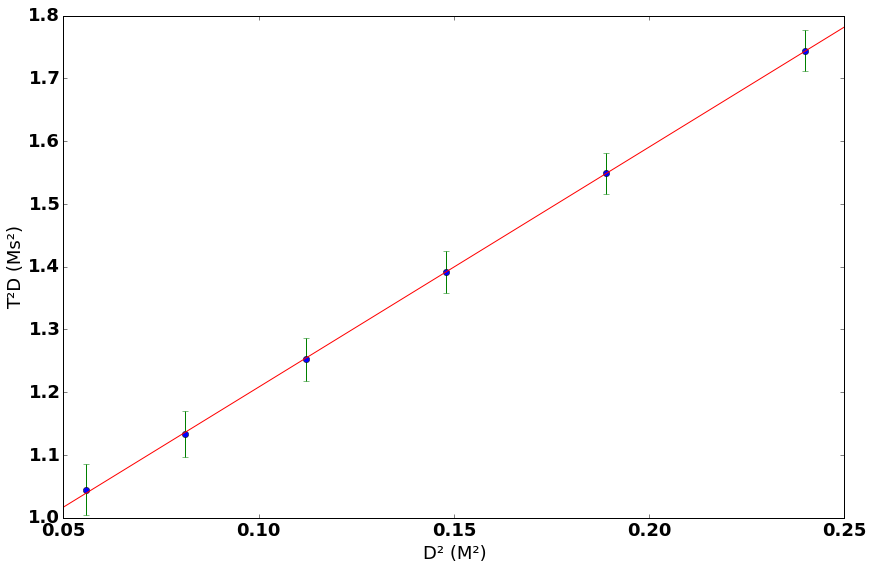
\includegraphics[scale=0.55]{index.png} 
\emph{Gráfico 1: $T^2D$ em função de $D^2$. Nota-se que os dados coletados se encaixam muito bem em uma projeção linear.}

\label{fig:Grafico}
\end{figure}
\subsection{Gravidade}
A interpretação física do coeficiente angular encontrado é, por (\ref{eq:funcao}),
 $$ a = \frac{4\pi^2}{g} = 3.8 \pm 0.2$$
  logo podemos encontrar $g$ como 

  $$ g = \frac{4\pi^2}{3.8} = 10.3 M/s^2 $$ 
  e seu erro associado, propagado a partir do erro em $a$ é
  $$ \Delta g = \frac{4\pi^2}{a^2} \cdot \Delta a = \pm 0.6 m/s^2 $$
  
\subsection{Raio de giração}

A interpretação física do coeficiente linear, a partir de (\ref{eq:funcao}), é 
$$ b = \frac{4\pi^2}{g} \cdot k^2 = 0.83 \pm 0.04 $$
logo, 
$$ k = \sqrt{\frac{g \cdot b}{4\pi^2}} = 0.46 $$
$$ \Delta k = \pm 0.02 $$

\subsection{Momento de Inércia}
O momento de inércia pode ser descrito em função do raio de giração como 
$$ I_{cm}  = Mk^2 $$
$$ I_{cm}  = 0.28 (M \cdot Kg)$$
E o erro $ \Delta I_{cm}$ pode ser calculado a partir da expressão 
$$\Delta I_{cm}  =\sqrt{(2mk \cdot \Delta k)^2 + (k^2 \cdot \Delta M)^2} = \pm 0.02 (m \cdot Kg) $$

\section{Conclusões}

\end{document}
